\SSbreak\\
\emph{Source: Original}\\
\emph{Proposer: \Ptan and \Pwen}\\
\emph{Problem ID: 155}\\
\emph{Date: 2021-03-09}\\
\emph{Difficulty: Beginner}\\
\SSbreak

\SSpsetQ{
    A circle with area $\frac{20}{21}$ is placed randomly in the plane. What is the probability that the circle will contain a lattice point? (Formally,
    if $p_M$ is the probability that a circle with center chosen randomly in $[-M, M]^2$ contains a lattice point, find $\lim_{M \to \infty} p_M$.)
}\bigskip

\begin{solution}\hfil\medskip
  
    By symmetry, it suffices to consider the probability when the circle's center is chosen randomly inside a unit square. Draw four quartercircular arcs,
    one at each vertex; such a circle's center must be contained in the union of those arcs in order for it to contain a lattice point (otherwise a lattice point
    would more more than $r$ away from the circle's center). Shown below is the diagram.

    \begin{center}
        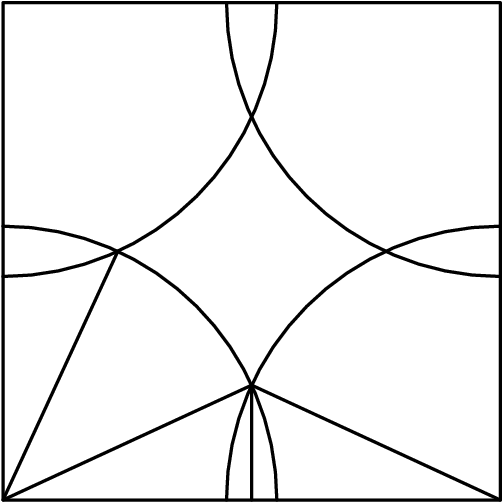
\includegraphics[width=7cm,height=7cm]{Sections/Files/11-2-1-img.png}
    \end{center}

    Since the arcs overlap, we split the area into four isosceles triangles and four arcs. The base angle of the triangle is $\arccos\left(\frac{1}{2r}\right)$
    and the height of the triangle is $\sqrt{r^2 - \frac{1}{4}}$ so the angle of the arc is $\frac{\pi}{2} - 2 \arccos\left(\frac{1}{2r}\right).$ Multiplying by
    four and plugging in $r = \sqrt{\frac{20}{21\pi}}$ we get
    $$P = \boxed{2 \sqrt{\dfrac{20}{21\pi} - \dfrac{1}{4}} + \dfrac{20}{21}\left(1 - \dfrac{4 \arccos\left(\frac{\sqrt{21 \pi}}{2\sqrt{20}}\right)}{\pi}\right)}.$$
\end{solution}\bigskip